\documentclass[a4paper,12ptc, dvipdfmx]{jsarticle} %文字サイズは変えても良い
\usepackage[dvipdfmx]{graphicx}
\usepackage{amssymb, amsmath}
\usepackage{url}
\usepackage{tikz}  
\usetikzlibrary{decorations.pathreplacing,calligraphy}
\usepackage{float}
\usepackage{setspace}
\usepackage[top=30truemm,bottom=30truemm,left=25truemm,right=25truemm]{geometry} % ページの設定
\pagestyle{empty} %ページ番号なし
%\setlength{\headheight}{0truemm}
%\setlength{\parindent}{1zw}
\makeatletter
\def\section{\@startsection {section}{1}{\z@}{.7ex plus .2ex minus .2ex}{.1 ex plus 1.2ex}{\normalsize\bf}}
\makeatother
\setstretch{0.9}

\begin{document}
%\twocolumn[ 
\begin{center}
{\bf \Large 非負値行列因子分解の統一的な拡張と医学データ解析}
\vspace{0.3em}
\begin{tabular}{rl}
\vspace{-0.1em} \bf 名古屋大学大学院医学系研究科 &  \bf 阿部興 \\
\vspace{-0.1em} \bf 名古屋大学大学院医学系研究科/東京医科歯科大学難治疾患研究所 &  \bf 島村徹平\\
\end{tabular}
\vspace{0.5em}
\end{center}
%]
\vspace{\baselineskip}

%\maketitle
\section{はじめに}
生命科学の分野においては, 次世代シークエンシングに代表される実験技術の進歩に伴い, ゲノム, エピゲノム, トランスクリプトーム, プロテオーム, メタボロームといった, 多数の要素を縦断的に観測することが可能になった. これらのデータは, 非負の整数(カウント)データである事が多く, 計算機上では多次元配列(テンソルと呼ばれることもある)を使用して表すことができる. そして, 環境因子と遺伝子型, 表現型との関連を明らかにするための豊富な情報を持つ. 一方で, データが高次元になるため, 多変量のデータの次元削減やパターンの抽出を行う分析手法の開発が求められている. 

多変量解析はかねてより研究されてきたテーマである. 主成分分析(Tipping \& Bishop, 1999), 潜在的ディリクレ配分(Blei \& Jordan, 2003), 非負値行列因子分解(NMF; Cemgil, 2009)といった, データの次元削減やパターンの抽出を行うことを目的とした統計モデルの多くは, 行列分解を行う手法と捉えることができる. 
テンソル分解は行列分解をさらに多次元へ拡張する方法の一つである. しかし, データを3次元以上の多次元配列に格納する場合, 繰り返し測定や補助的な情報がある場合にその都度データの形式を作り変える必要がある. また, 欠損値がある場合には, 欠損をなんらかの方法で補完する, または欠損した部分をマスクするといった処理が必要になる. 

これに対して, tidy data と呼ばれる次の条件を満たす形式でデータを取り扱うことが提唱されている (Wickham, 2019).
\begin{enumerate}
     \item 各変数が 1 つの列を形成する
     \item 各観測値が 1 つの行を形成する
     \item 各観測の観測単位の種類が 1 つのテーブルを形成する
     \item 各値が 1 つのセルを構成する
\end{enumerate}
tidy data の形式でデータを処理する場合, 繰り返し測定はテーブルへの行の追加, 欠損はテーブルからの行の削除であり, 大規模な変更は起こらない. 
さらに, 実験時の条件や補助的な情報を列として, あわせて分析することができる.

Abe \& Shimamura (2023) ではNMFを tidy data の枠組みに拡張し, 多次元のデータを柔軟に分析するモデル,  unified non-negative matrix factorization (UNMF) を提案した.本報告ではこのモデルを活用し, 数値実験とデータ分析の結果を示す.

\section{モデルと推定アルゴリズム}

UNMF は, 因子分解と同様に, 潜在因子と観測された変数間の関係を記述する. 観測された$y=(y_1,\ldots, y_N)'$および計画行列 $X=(x_{nd})$ ($x_{nd} \in \{0,1\}$) に対し, UNMF は次のような $D \times L$ の非負値行列 $V = (v_{dl})$ を推定する.
\begin{align*}
y_{n} \approx \sum_{l=1}^L \prod_{d=1}^D v_{dl}^{x_{nd}}.
\end{align*}
ここで, $D$ は $X$ の次元(列の数)によって定まり,  $L$ はユーザーが指定する. 行列 $V$ は $y_n$ の共起関係を記述するパラメータである. 右辺は $X$ の非ゼロ成分で指定される $V$ の行ベクトルのなす方向どうしが近いときより大きく, 遠いときにはより小さい値となる.

\begin{figure}
\begin{tikzpicture}[scale=0.9]
\def\rxo{4}
%brace
\draw [decorate, decoration = {brace}, thick] (-0.25, 0) --  (-0.25, 5) node [midway, left, xshift=-2pt]{$N$}; %y
\draw [decorate, decoration = {brace, mirror}, thick] (\rxo, -4.25) --  (\rxo+5, -4.25) node [midway, below, yshift=-2pt]{$D$}; 
\draw [decorate, decoration = {brace, mirror}, thick] (\rxo+5.25, -4) --  (\rxo+5.25, -2) node [midway, right, xshift=+2pt]{$L$}; %V
%matrix
\draw[step=1cm, black, thick] (1, 5) grid (0,0); %y
\draw[step=1cm, black, thick] (\rxo+5, 5) grid (\rxo,0); %X
\draw[step=1cm, black, thick] (\rxo, -2) grid (\rxo+5, -4); %V

\draw [decorate, decoration = {brace, mirror}, thick] (\rxo, -0.1) --  (\rxo+1.95, -0.1) node [midway, below]{被験者}; %below X
\draw [decorate, decoration = {brace, mirror}, thick] (\rxo+2.05, -0.1) --  (\rxo+5, -0.1) node [midway, below]{項目}; %below X

%label
\node[draw, circle, color=white, fill=gray] (Y) at (0.5, 5.5) {\Large $y$};
\node[draw, circle,  color=white, fill=gray] (X) at (\rxo+2.5, 5.5) {\Large $X$};
\node[draw, circle, black] (V) at (\rxo+2.5, -1.4) {\Large $V'$};
%fill Y
\foreach \x in {0, 1, 3} \draw[fill=gray] (0, \x) rectangle ++(1,1);
% fill X
\foreach \x in {(\rxo, 0), (\rxo,4), (\rxo+1,3), (\rxo, 2), (\rxo+1, 1)} \draw[fill=gray] \x rectangle ++(1,1);
\foreach \x in {(\rxo+4, 0), (\rxo+2,4), (\rxo+2, 3), (\rxo+3,2), (\rxo+3,1)} \draw[fill=gray] \x rectangle ++(1,1);
%fill V
\foreach \x in {(\rxo,-4), (\rxo+1, -3), (\rxo+2,-3), (\rxo+3,-3), (\rxo+4,-4)} \draw[fill=gray] \x rectangle ++(1,1);
%dummy node
\node (dY) at (1.2, 2){};
\node (dX) at (\rxo-0.1, 2){};
\node (dV) at (\rxo, -2){};
\draw[->, thick] (dX)--(dY) node[midway, above]{\large $\displaystyle \sum_{l=1}^{L}\prod_{d=1}^D v_{dl}^{x_{nd}}$};
\draw[->, thick] (dV)--(dY);
%%
%Y matrix
\draw[step=1cm, black, thick] (\rxo+7, 0) grid (\rxo+9,2);
\draw[step=1cm, black, thick] (\rxo+9, 1) grid (\rxo+10,2);
\foreach \x in {0,1} \draw[fill=gray] (\rxo+\x+7, 0) rectangle ++(1,1);
\draw[fill=gray] (\rxo+2+7, 1) rectangle ++(1,1);
%%
%V matrix
\draw[step=1cm, black, thick] (\rxo+7, -2) grid (\rxo+9, -4); %left
\foreach \x in {(\rxo+7,-4), (\rxo+8, -3)} \draw[fill=gray] \x rectangle ++(1,1);
\draw[step=1cm, black, thick] (\rxo+10, -2) grid (\rxo+13, -4); %right
\foreach \x in { (\rxo+10,-3), (\rxo+11,-3), (\rxo+12,-4)} \draw[fill=gray] \x rectangle ++(1,1);
%label (right)
\draw[rounded corners, dashed]  (\rxo+6.5, 3) rectangle (\rxo+14, -4.5);
\node[rotate=90] (app) at (\rxo+9, -0.7){\Huge $\approx$};
\node (times) at (\rxo+9.5, -3){\Huge $\times$};
\node (Ym) at (\rxo+11.5, 1.5) {{\Large $Y$} ($\mathrm{vec}(Y)=y$)};
\node (V) at (\rxo+8, -1.5) {\Large $V_{(1)}$};
\node (V) at (\rxo+11, -1.5) {\Large $V'_{(2)}$};
\node (plate) at (\rxo+9.5, 2.5) {等価な行列分解};
\end{tikzpicture}
\caption{UNMFの視覚的な例. 灰色の円は観測された変数を示し, 白は潜在変数 \label{mprod}.}
\end{figure}

UNMF を使用した tidy data 形式での行列分解を, 簡単な例を通じて紹介する (図 \ref{mprod}). 2人の被験者に対し実験で 3 つの項目の観測値が得られたとする. 実験の結果得られたデータは行で被験者, 列で項目を区別して, 行列$Y$で表すことができる. 一方, 実験の結果得られたデータをベクトル $y = \mathrm{vec}(Y)$ に対し, 行列 $X$ を被験者と項目を表すダミー変数で表現することもできる. これは tidy data の形式と直接対応する. 行列で表現したときと tidy data の形式で表現したときとで, データの持つ情報は等しい. UNMF は次の式が成り立つように推定を行う.
\begin{align*}
y_{n}  \approx \sum_{l=1}^L \prod_{d=1}^D v_{dl}^{x_{nd}} = V_{(1)}V_ {(2)}'
\end{align*}
右辺より, この場合UNMFはNMFと等価である. ここで $V_{(1)} = (\prod_{d=1}^2 v_{dl}^{x_{nd}})$, $(V_{(2)} = \prod_{d=3}^5 v_{dl}^{x_{nd}}) $ とした.

図 \ref{mprod} では$Y$の(2,3)成分が欠損した状況を示している. この場合もUNMFの枠組みではデータに対し特殊な処理は必要とされない. また, 同一条件の重複(繰り返し測定)がある場合も同様である. さらに, 被験者と項目のみならず,  観測した時点やその他の説明変数といった, 豊富な情報を含むデータが得られている場合を含め, 一貫した枠組みで分析を行うことができる.

さて, 具体的な確率モデルとして, UNMFは次のデータ生成過程を考える.
\begin{align}
y_{n} \mid v_{dl}, x_{n} & \sim \mathrm{Poisson}\left(\sum_{l=1}^{L} \left\{\prod_{d=1}^{D}v_{dl}^{x_{nd}} \right\} \right),  \label{geney}\\
v_{dl} & \sim \mathrm{Gamma}(a,b).\nonumber
\end{align}
ここで $\mathrm{Poisson}(\lambda)$ は平均 $\lambda$ のポアソン分布, $\mathrm{Gamma}(a,b)$ は形状パラメータ $a$, レートパラメータ$b$ のガンマ分布, およびそれらの確率密度を意味する. ガンマ分布はパラメータ$V$に対する事前分布として置いた. 

式 (\ref{geney}) は次の表現と等価である.
\begin{align*}
y_{n}  = \sum_{d=1}^{D} \sum_{l=1}^{L}u_{nl}, \quad u_{nl} \sim \mathrm{Poisson}\left(\prod_{d=1}^{D}v_{dl}^{x_{nd}} \right)
\end{align*}
$u_{nl}$ は推定アルゴリズムを導くための補助的な潜在変数である. 
平均場近似の仮定, すなわち推定の対象となる変数の事後分布がすべて互いの独立であると仮定すると, いくつかの計算から, 事後分布の近似 $q(u_{nl})$ および $q(v_{dl})$を得ることができる (Jordan, \textit{et al.}, 1999). すなわち, 潜在変数が互いに独立だとした範囲内で, カルバック・ライブラ距離の意味で事後分布に近い分布を求めるという, 変分ベイズ法による推定を行う. 表記として, ある確率変数 $w$ に対し, その近似事後分布 $q(w)$ で評価した平均を $\widetilde w$ とする. また, 一般には $\log \widetilde w $ と$\widetilde{\log w}$ は一致しないことに注意する. $q(u_{nl})$ は次に示すパラメータ $r_{nl}$ を持つ多項分布,
\begin{align}
r_{nl} =\frac{\exp(\widetilde{\log v_{dl}})}{\sum_{l=1}^{L} \exp( x_{nd} \widetilde{\log v_{dl}} ) },
\label{eqPostMulti}
\end{align}
$q(v_{dl})$は次に示す形状パラメータ $\hat a_{dl}$, レートパラメータ $\hat b_{dl}$ のガンマ分布である.
\begin{align}
\hat a_{dl} &= \sum_{n=1}^{N} \sum_{n=1}^{N}x_{nd} \widetilde{u_{nl}} + a, \nonumber \\
\hat b_{dl} &= \sum_{n=1}^{N} x_{nd}  \left( \prod_{d' \neq d} \widetilde{v_{d'l}}^{x_{nd'}} \right) + b.
\label{eqPostGamma}
\end{align}

推定アルゴリズムは次の手順としてまとめられる.
\begin{itemize}
   \item $v_{dl}$ をガンマ分布で初期化する
    \item 指定された反復回数まで次のステップを繰り返す
    \begin{itemize}
    \item 式 (\ref{eqPostMulti}) を用いて $\widetilde{u_{nl}}$ を更新
    \item 式 (\ref{eqPostGamma}) を用いて $\widetilde{v_{dl}}$ と $\widetilde{\log v_{dl}}$ を更新
    \end{itemize}
\end{itemize}

%次に, ポアソン分布以外の分布によるモデル化について考える. 離散(カテゴリカル)データのモデルによく使われる代表的な確率分布として, 多項分布や

\section{分析対象}
本研究ではシークエンシングと呼ばれる技術を利用して得られたデータを主な分析の対象とする. これらはサンプルから得られる塩基配列を化学的に増幅して標識し, 塩基を特定する. 結果, 得られるのは塩基配列ごとのカウントデータである. この技術は, DNAの塩基配列を元に, 合成されたRNAから組織ごとに発現している遺伝子を特定するトランスクリプトーム解析, ある環境中から採取したサンプルにどのような種類の微生物が存在するかを調査するメタゲノム解析といった, 幅広い応用範囲を持つ. 

本稿では一例としてメタゲノム解析について記載する. David \textit{et al.} (2014) は、A と B の 2 人のドナーの糞便から採取したメタゲノムを縦断的に調査した.  ドナー B については, 530 種の細菌(不明な種は``unknown" としてまとめて集計)が 176 の時点で記録されており, ドナー B は 151日目から159 日目の間に腸管感染症に罹患していたことがわかっている.

我々は時間と菌種をワンホットエンコーディングでダミー変数とし, UNMFを用いてこのデータを分析した. データをホールドアウトしたバリデーションにより, $L=5$と定めた. 推定された$V$の近似事後分布による平均について, 図 \ref{Vplot} に示す. 図2が示すように, 150から160日目にかけて, 成分 4 は顕著に大きい値を取る. この成分 4 は, 食中毒の原因となることが知られている \textit{Eshtishia/Shigella}, \textit{Salmonella}, および \textit{Clostridium} 属によって特徴付けられる. このことは, UNMFによって背景知識と一致する特徴が抽出されたことを意味する. 
加えて, 成分4と入れ替わるように成分3が増加し, 腸管感染症以前に多くの割合を占めていた他の成分は減少した傾向が見て取れる. UNMFはこのように腸内細菌叢の変化を捉えることができる. 

\begin{figure}
\centering
\begin{tabular}{c}
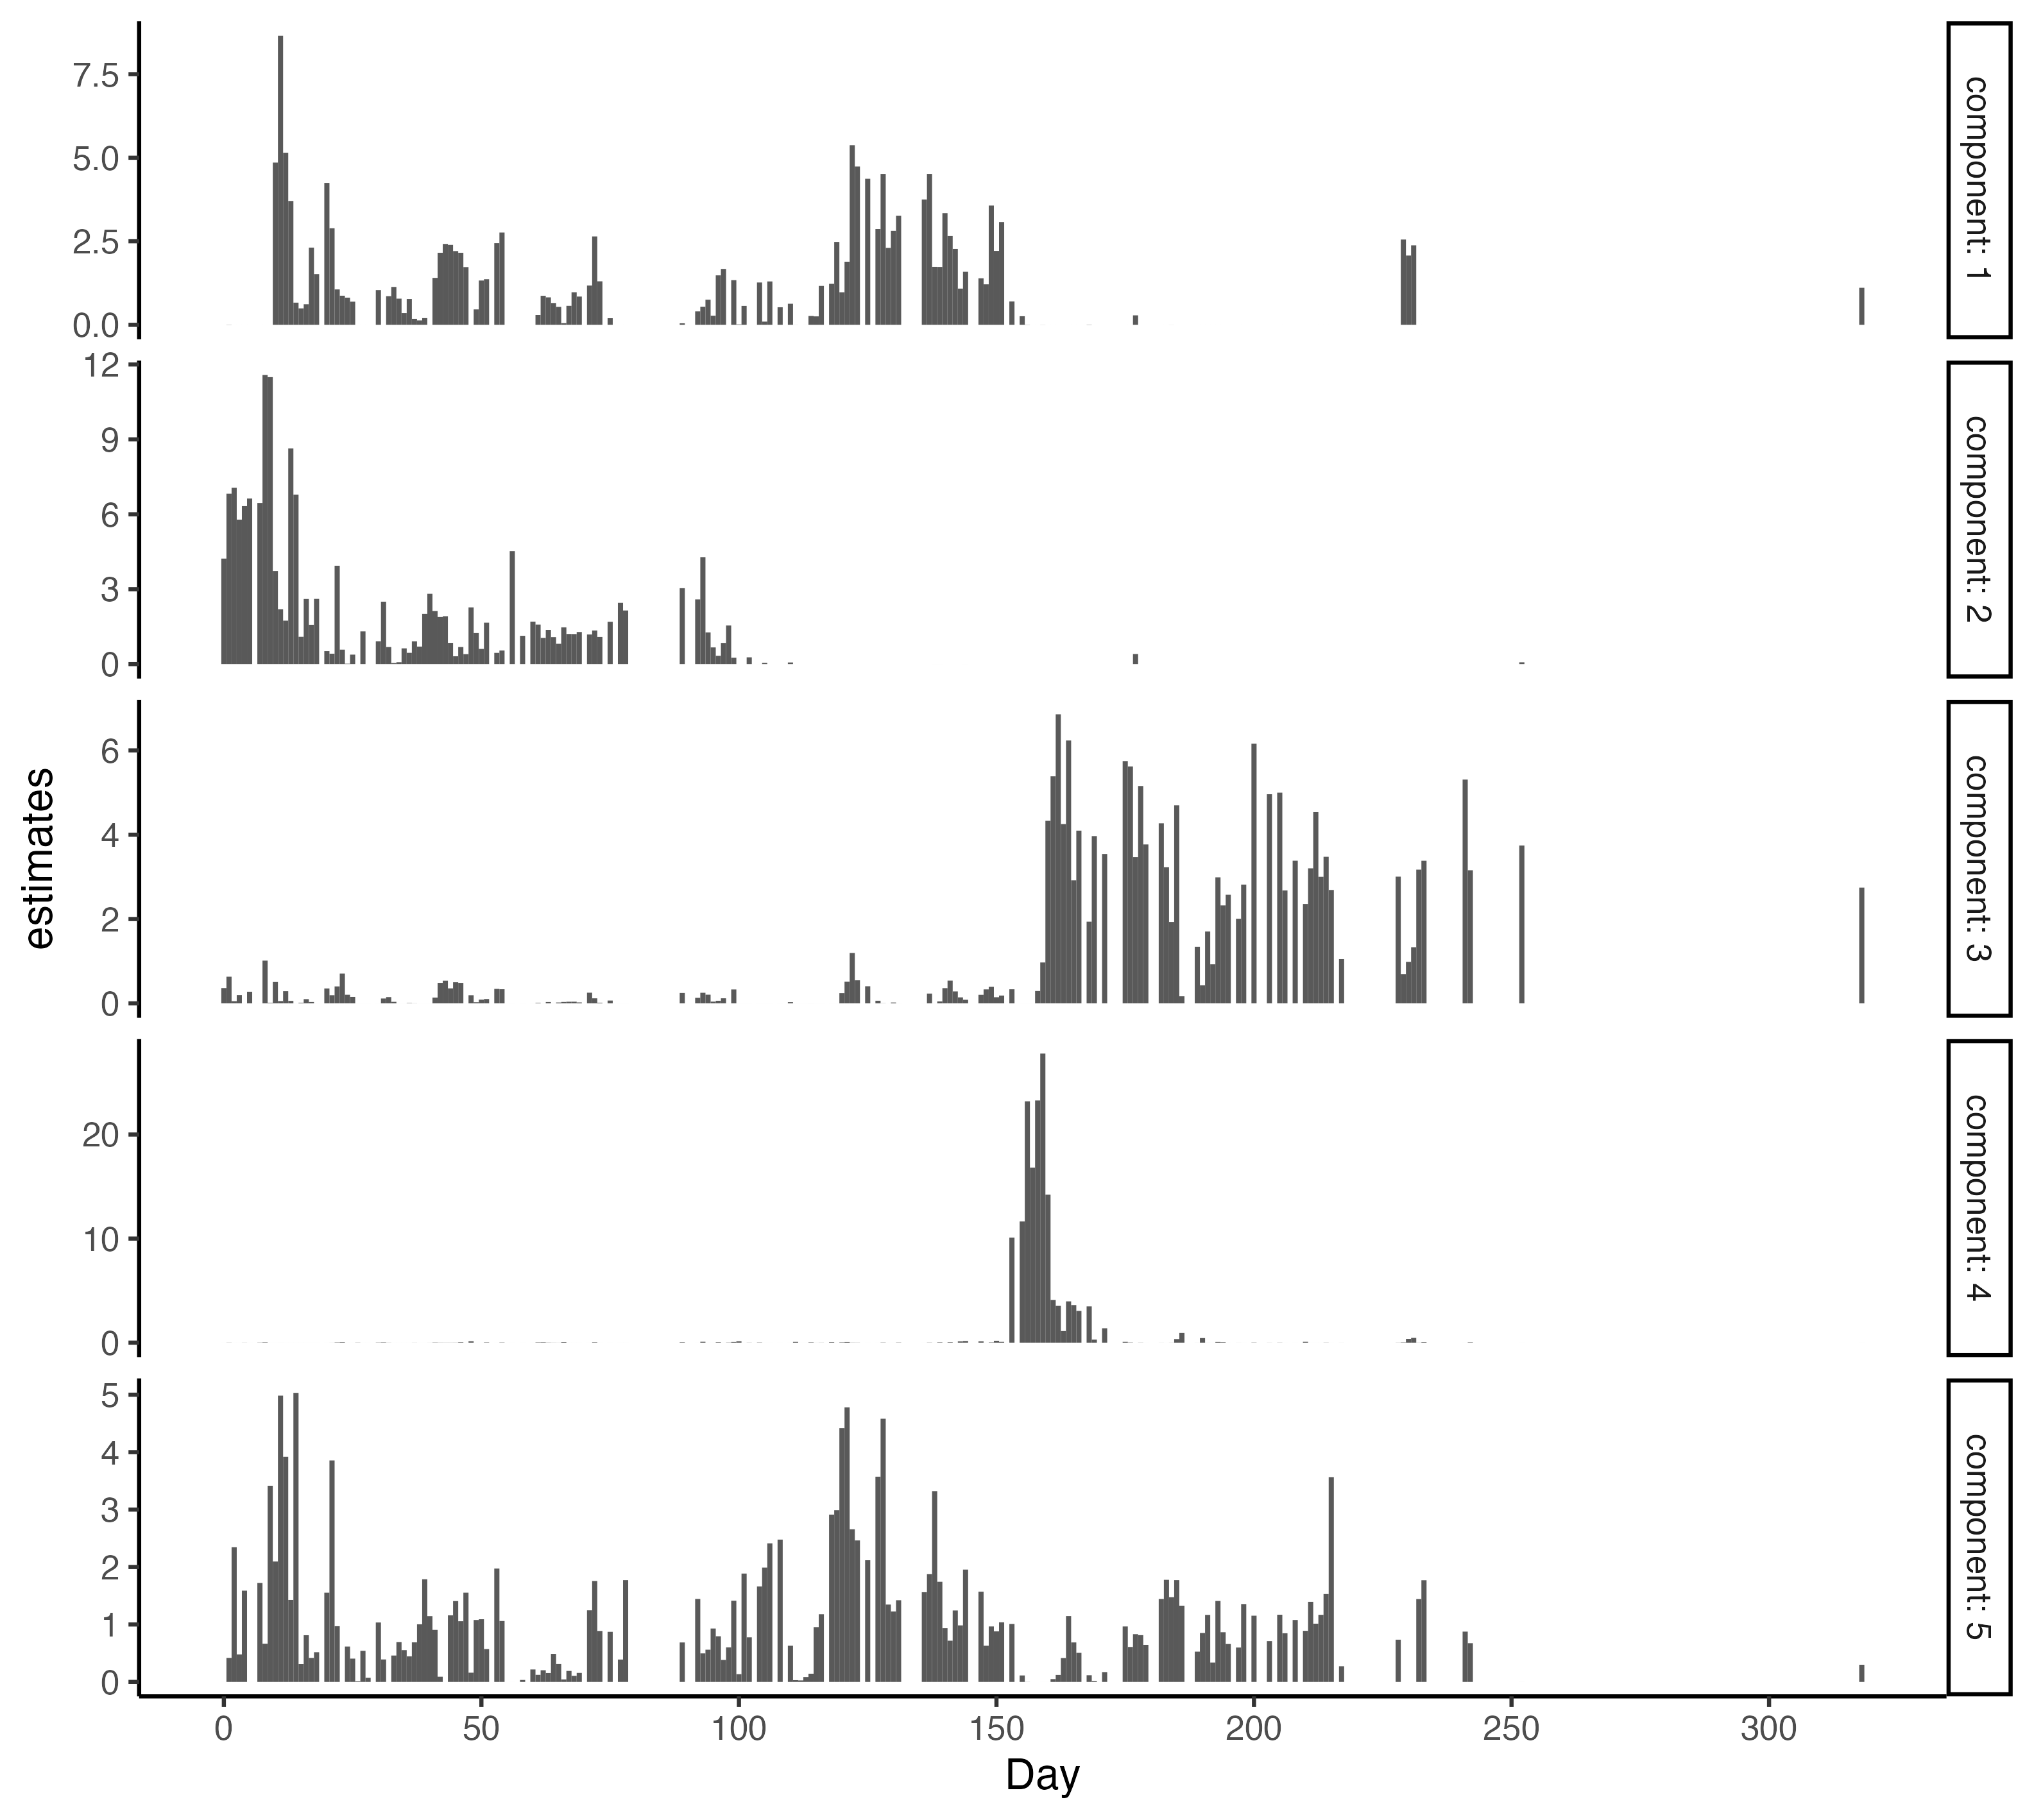
\includegraphics[width=10cm]{david_day.png} \\
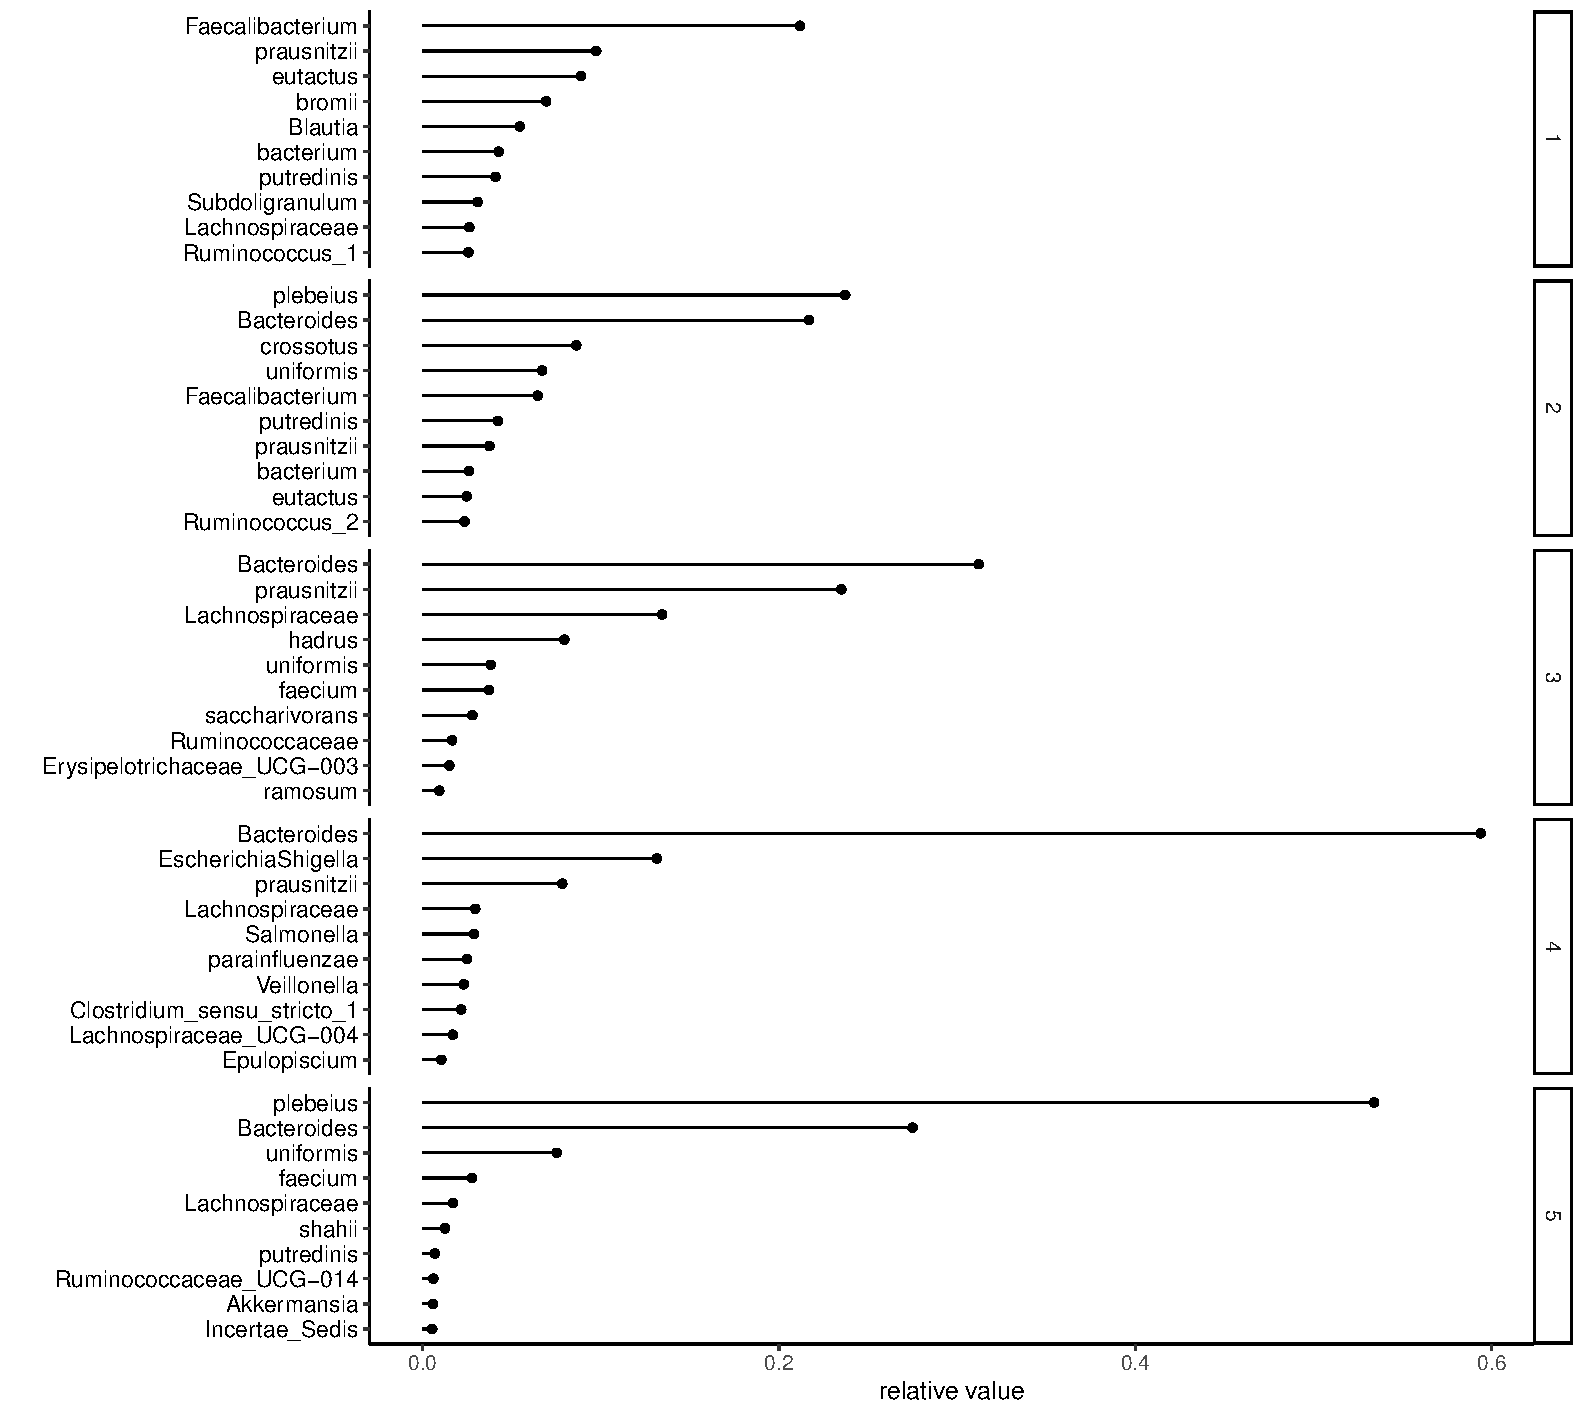
\includegraphics[width=10cm]{david_genus.pdf}
\end{tabular}
\caption{推定された$V$. 上段:時間ダミー, 下段:菌種ダミーに対応する. 下段では代表的な細菌上位10種のみを示した.\label{Vplot}}
\end{figure}

大会ではこれらのデータ分析事例に合わせて数値実験の結果を報告する.

\begin{thebibliography}{9}
\bibitem{Tipping} Tipping~ME., \& Bishop, CM. (1999).  Probabilistic principal component analysis. {\em Journal of the Royal Statistical Society: Series B (Statistical Methodology)}, 61(3), 611-622.
\bibitem{Blei} Blei DM, Ng AY, \& Jordan MI. (2003). Latent dirichlet allocation. {\em Journal of machine Learning research}, 3(Jan), 993-1022.
\bibitem{Cemgil} Cemgil~AT. (2009).  Bayesian inference for nonnegative matrix factorisation models. {\em Computational intelligence and neuroscience}, 2009.  \url{https://doi.org/10.1155/2009/785152}
\bibitem{Wickham2019} Wickham H. (2019).  {\em Advanced R, second edition}. Chapman and Hall/CRC.
\bibitem{AbeShimamura} Abe K \& Shimamura T. (2023). UNMF: A unified non-negative matrix factorization for multi-dimensional omics data. {\em Briefings in Bioinformatics.} (Under Review).
\bibitem{Jordan} Jordan~MI, Ghahramani~Z, Jaakkola~TS \& Saul~LK. (1999). An introduction to variational methods for graphical models. {\em Machine learning}, 37(2), 183-233.
\bibitem{David} David LA, Materna AC, Friedman J, \textit{et al.} (2014). Host lifestyle affects humanmicrobiota on daily timescales. {\em Genome Biology}, 15(R89). \url{https://doi.org/10.1186/gb2014-157-r89}.
\end{thebibliography}
\end{document}  m 